%************************************************
\chapter{Filter Bank Common Spatial Patterns and
Filterbank Network}\label{ch:fbscp-and-filterbank-net}
%**************************************

\todotext{textbox}


    In a prior master thesis
\citep{schirrmeister_msc_thesis_2015}, we had developed a
neural network architecture closely resembling the feature-based
decoding algorithm filter bank common spatial patterns. In this chapter,
I describe filter bank common spatial patterns as well as the
corresponding filter bank network of the prior master thesis as the
starting point for the network architectures developed in the context of
this thesis.

\section{Filter Bank Common Spatial Patterns as a Starting
Point}\label{filter-bank-common-spatial-patterns-as-a-starting-point}


We selected filter bank common spatial patterns (FBSCP
\cite{ang_filter_2008,chin_multi-class_2009}) as the
feature-based EEG-decoding algorithm we were trying to imitate in our
initial neural network architectures. FBCSP is an EEG-decoding algorithm
that has been successfully used in task-related EEG-decoding
competitions \cite{tangermann_review_2012}. FBCSP aims to
decode task-related changes in signal amplitude in different
frequencies, such as a decrease in the amplitude of alpha and beta-band
oscillations during movement imagination. In the following, we will
explain how FBCSP decodes two classes of EEG signals by finding
frequency-specific spatial filters that transform the signal, such that
the transformed signal has relatively high variance for one class and low variance for the
other class and vice versa.


\section{Common Spatial Patterns}\label{common-spatial-patterns}


\begin{figure}[th]
    \myfloatalign
    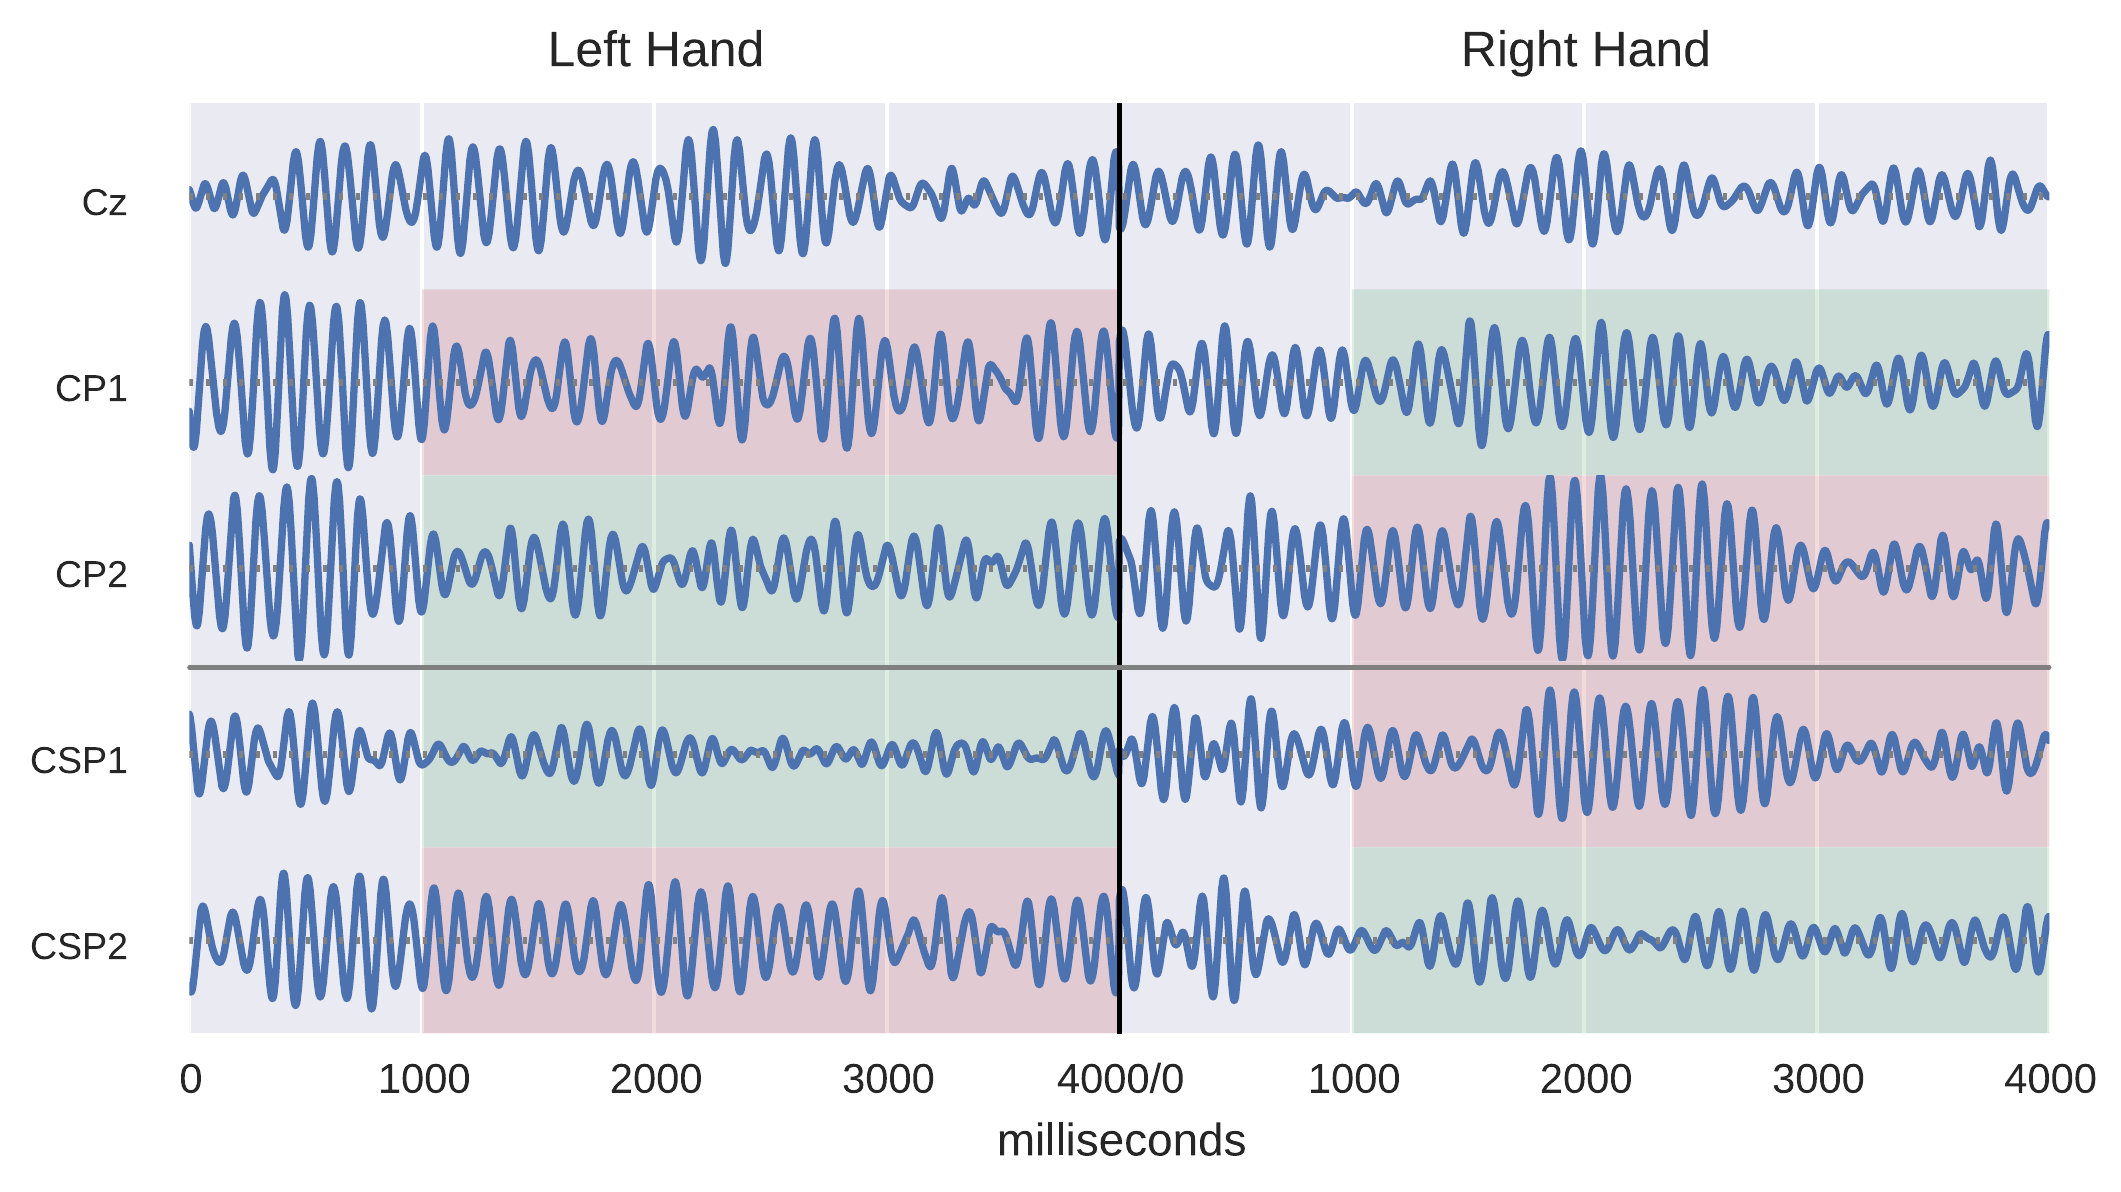
\includegraphics[width=1\linewidth]{images/Methods_Common_Spatial_Patterns_18_0.png}
    \caption[Common Spatial Patterns example.]{
\textbf{Common Spatial Patterns example.} Top parts show EEG
signals for three electrodes during a left hand and a right hand
movement. Bottom parts show spatially filtered signals of two CSP
filters. Green parts have lower variance and red parts have higher
variance. Note that this difference is strongly amplified after CSP
filtering. Figure from prior master thesis
\citep{schirrmeister_msc_thesis_2015}.}\label{csp-figure}
\end{figure}


    The basic building block of FBCSP is the common spatial patterns (CSP)
algorithm. CSP is used to decode neuronal activity that leads to a
change in the amplitudes of the EEG signal with a specific spatial
topography \citep{koles_spatial_1990,ramoser_optimal_2000,blankertz_optimizing_2008}.
To do that, CSP aims to maximize the ratio of the signal variance
between spatially filtered signals of two classes, e.g.~of the signal
during two different movements. For example, the signal of a spatial
filter computed by CSP may have a very large variance during movements
of the left hand and a very small variance during movements of the right
hand. Concretely, we are given signals
$X_{1}, X_{2} \in \mathbb{R}^{n x k x t}$ from $n$ EEG trials (can
be different for $X_1, X_2$, $k$ EEG electrodes and $t$
timepoints within each trial. CSP then finds a spatial filter $w$ that
maximize the ratio of the variances of the spatially filtered
$X_1,X_2$:

\begin{equation*}
w=\argmax_w\frac{Var(w^T X_1)}{Var(w^T X_2)}= \argmax_w\frac{||w^T X_1||^2}{||w^T X_2||^2}=\argmax_w\frac{w^T X_1 X_1^T w}{w^T X_2 X_2^T w}
\end{equation*}

    Rather than just finding a single spatial filter $w$, CSP is typically
used to find a whole matrix of spatial filters $W^{kxk}$, with spatial
filters ordered by the above variance ratio and orthogonal to each
other. The first filter $w_1$ results in the largest variance ratio
and the last filter $w_k$ results in the smallest variance ratio.
Different algorithms can then be used to subselect some set of filters
to filter signals for a subsequent decoding algorithm.

The CSP-filtered signals can be used to construct features to train a
classifier. Since the CSP-filtered signals should have very different
variances for the different classes, the natural choice is to use the
per-trial variances of the CSP-filtered signals as features. This
results in as many features per trial as the number of CSP filters that
were selected for decoding. Typically, one applies the logarithm to the
variances to get more standard-normally distributed features.


\section{Filter Bank Common Spatial
Patterns}\label{filter-bank-common-spatial-patterns}

    CSP is typically applied to an EEG signal that has been bandpass
filtered to a specific frequency range. The filtering to a frequency
range is useful as brain signals cause EEG signal amplitude changes that
are temporally and spatially different for different frequencies
\citep{ang_filter_2008}. For example, during movement the
alpha rhythm may be suppressed for multiple electrodes covering a fairly
large region on the scalp while the high gamma rhythm would be amplified
for a few electrodes covering a smaller region.

    Filter bank common spatial patterns applies CSP separately on signals
bandpass-filtered to different frequency ranges
\cite{ang_filter_2008,chin_multi-class_2009}. This allows
to capture multiple frequency-specific changes in the EEG signal and can
also make the decoding more robust to subject-specific signal
characteristics, i.e., which frequency range is most informative for a
given subject. The trial-log-variance features of each frequencyband and
each CSP filter are then concatenated to form the entire trial feature
vector. Typically, a feature selection procedure will select a subset of
these features to train the final classifier.

    The overall FBCSP pipeline hence looks like this:

\begin{enumerate}
\def\labelenumi{\arabic{enumi}.}
\item
  \textbf{Bandpass filtering}: Different bandpass filters are applied to
  separate the raw EEG signal into different frequency bands.
\item
  \textbf{Epoching}: The continuous EEG signal is cut into labeled
  trials, e.g., 4-second left-hand or right-hand movement windows.
\item
  \textbf{CSP computation}: Per frequency band, the common spatial
  patterns (CSP) algorithm is applied to extract spatial filters (see
  \Cref{common-spatial-patterns}).
\item
  \textbf{Spatial filtering}: The spatial filters computed in Step 2 are
  applied to the EEG signal.
\item
  \textbf{Feature construction}: Feature vectors are constructed from
  the filtered signals: Specifically, feature vectors are the
  log-variance of the spatially filtered trial signal for each frequency
  band and for each spatial filter.
\item
  \textbf{Feature selection}: A feature selection algorithm may be used
  to only retain a subset of the features for classification.
\item
  \textbf{Classification}: A classifier is trained to predict per-trial
  labels based on the feature vectors.
\end{enumerate}

\section{Filter Bank Network
Architecture}\label{filter-bank-network-architecture}


\begin{figure}[th]
    \myfloatalign
    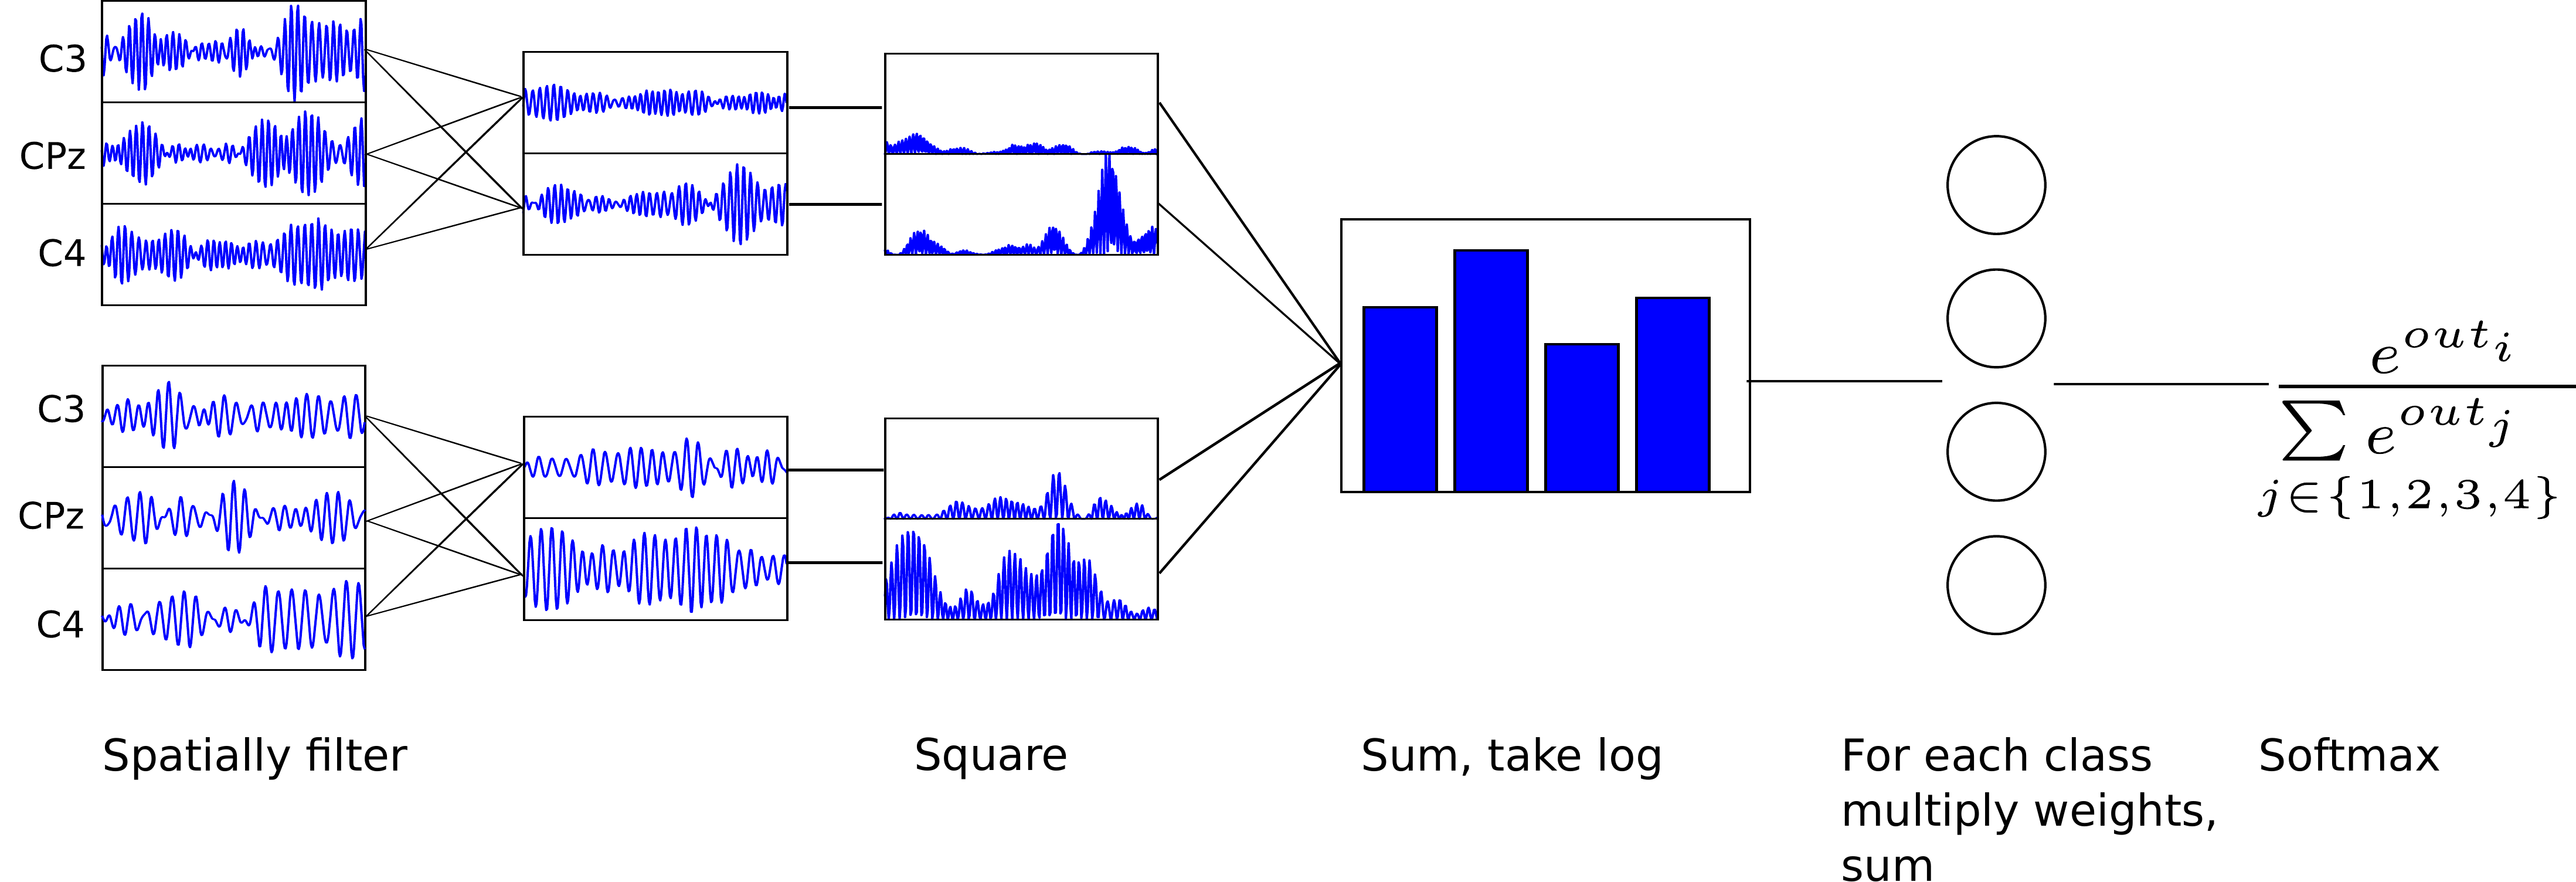
\includegraphics[width=1\linewidth]{images/csp_as_a_net_explanation.png}
    \caption[Filter bank network architecture overview.]{
\textbf{Filter bank network architecture overview.} Input signals were
bandpass filtered to different frequency ranges. Signals are first
transformed by learned spatial filters, then squared, summed and the
log-transformed. The resulting features are transformed into class
probabilities by a classification weights followed by the softmax
function. Figure taken from a master thesis
\citep{schirrmeister_msc_thesis_2015}.}\label{filterbank-net-figure}
\end{figure}


    The first neural network architecture was developed by us in a prior
master thesis \citep{schirrmeister_msc_thesis_2015} to
jointly learn the same steps that are learned separately by FBCSP (see
\Cref{filterbank-net-figure}). Concretely, the network
simultaneously learn the spatial filters across many frequency bands and
the classification weights for the log squared sums of all resulting
spatially filtered signals. To be able to do that, the network is fed
with input EEG signals that were bandpass-filtered to different
frequency ranges. The network then performs the following steps:




\begin{align*}
    \intertext{\textbf{Spatial Filtering}}
    h_1 &= W_s^Tx && \color{commentcolor}{\small \text{Apply spatial filter weights } W_s \text{ to  inputs }} \\
    \intertext{\textbf{Feature Construction}}
    h_2 &= h_1^2 && \color{commentcolor}{\small \text{Square the spatially filtered signals }} \\
    h_3 &=\sum_t (h_2) && \color{commentcolor}{\small \text{Sum the squared signals across trial timepoints } t} \\
    h_4 &= \log(h_3) && \color{commentcolor}{\small\text{Take the logarithm of the summed values}}\\
    \intertext{\textbf{Classification}}
    h_5 &= W_c^Th_4 && \color{commentcolor}{\small \text{Apply classifier weights } W_c \text{ on these features }} \\
    p(c_i|h_5) &= \frac{e^{h_{5,i}}}{\sum_j e^h_{5,j}} && \color{commentcolor}{\small \text{Take the softmax to compute class probabilities}} \\
\end{align*}

    The spatial filter weights and the classification weights are trained
jointly.

\todotext{textbox}
